\section{Evaluation}
This section describes the in-depth analysis of 16 micro-benchmark experiments.
The experiments are partitioned into four sections; single core/multi-core and TCP/UDP.
On single core we evaluate TX/RX and RR on multi-core we evaluate TX/RX and Bi-Directional traffic.

\subsection{Summery of Results}
Tables ~\ref{tab:exec-single} and summersize the micro-benchmark results and analysis.
\begin{table*}
\centering
\begin{tabular}{l|c|c|c}
Experiment & vanilla & \oursys & reason\\\hline
Single UDP TX (Gb/s)& 44 & 52 (+18\%) &  instructions per packet\\
Single UDP RX & 90 & 52 & Faulty experiment\\
Single UDP RR (60B pps)& 186k & 195k(+4.8\%) & see discussion\\\hline
Single TCP TX (Gb/s)& 60.33 & 62.45 (+3.5\%) & Need manual inspection\\
Single TCP RX (Gb/s)& 55.3 & 56.48 (+2.7\%)& slightly better IPC\\
Single TCP RR (pps)& 176.6 & 185.2 (+5.1\%)& instructions per packet\\\hline
\end{tabular}
\caption{\label{tab:exec-single}Single core results breakdown.}
\end{table*}
\begin{table*}
\centering
\begin{tabular}{l|c|c|c}
Experiment & vanilla & \oursys & reason\\\hline
Multi UDP TX (Gb/s|CPU)& 147 | 100\% & 200 | 50\% &  Locking issues in vanilla\\
Multi UDP RX (Gb/s|CPU)& 200 | 40\%  & 200 | 40\% & Equal results\\
Multi UDP BI (Gb/s|CPU)& 240 | 100\% & 360 | 88\% &Locking in vanilla, \oursys limited by mem BW\\\hline
Multi TCP TX (Gb/s)& 187.41|39.7\% & 187.7|37.37\% & (+6.4\%)better instructions per packet - (alloc\_skb)\\
Multi TCP RX (Gb/s)& 200|46\% & 200|46\%& Equal results\\
Multi TCP BI (pps)& 350|64.13\% & 350|61.29\%& Not clear why 400Gb/s not reached\\\hline
\end{tabular}
\caption{\label{tab:exec-multi}Multi-core results breakdown.}
\end{table*}
\subsection{Methodology}
We count the average cycles per function using perf. The changes needed or \oursys were integrated in just a few places. table lists these locations.

\begin{table*}
\centering
\begin{tabular}{l|c|c}
name & location & expected impact \\\hline
mlx5e\_post\_rx\_wqes & mlx5 napi handler(IRQ) & RX\\
\_\_alloc\_skb & net\/core & TX\\
alloc\_skb\_with\_frags & TCP IN & TX\\
skb\_page\_frag\_refill & net\/core & TX\\
\_\_free\_pages & mem & all\\
skb\_free\_head & mem & all\\
alloc\_skb\_with\_frags & net\/core & TX\\
sock\_\{dev\_\}wmalloc & IP OUT(\_\_ip\_append\_data) & TX\\
sock\_\{dev\_\}alloc\_send\_pskb & IP OUT(\_\_ip\_append\_data)& TX\\
sk\_stream\_alloc\_skb & TCP & TX\\
\_\_netdev\_alloc\_skb & core & TX\\
\_\_napi\_alloc\_skb & core & TX\\
skb\_copy* & core & TX \\
skb\_segment & core & TX\\
\hline
\end{tabular}
\caption{\label{tab:func_list}Modified Functions}
\end{table*}

\subsubsection{TX}
On TX the send process starts from a system call, and then each message goes trough three phases; I routing + skb allocation II Copy and checksum and III udp send. We change the skb allocation function only. 

\subsection{Single-core UDP}
All single core tests are aimed to utilize 100\% of the CPU. In UDP-TX we have a single netperf flow sending 63KB datagrams. Using a dedicated memory allocator, boosts performance by 17.4\% in single core UDP TX experiment.

\begin{figure}
\centering
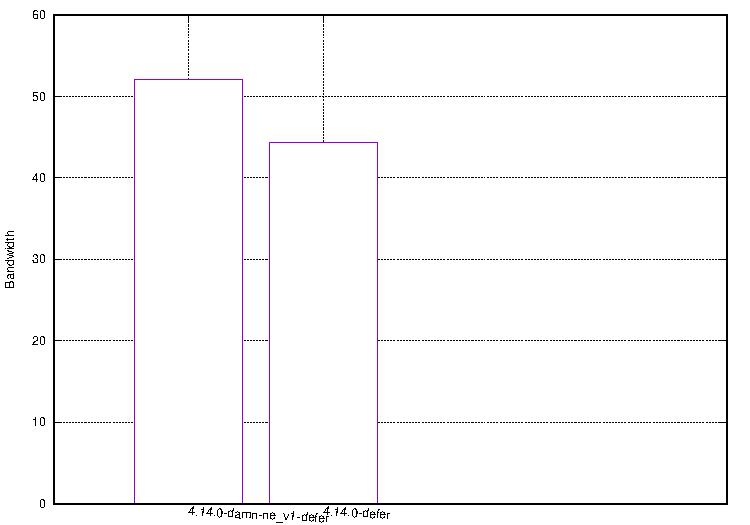
\includegraphics[width=0.5\textwidth]{figures/single_udp_tx_Bandwidth.pdf}
\caption{\label{fig:s-u-tx} Dan, I know that the text on the graph is too small. Single-core UDP TX.}
\end{figure}

\begin{figure}
\centering
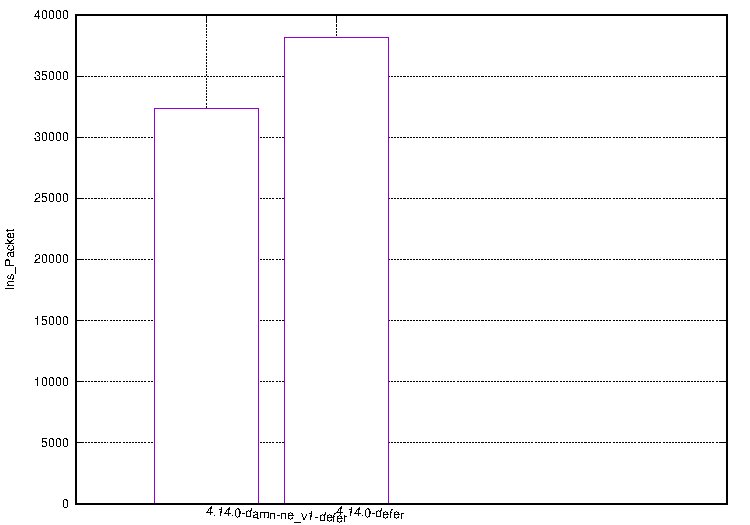
\includegraphics[width=0.5\textwidth]{figures/single_udp_tx_Ins_Packet.pdf}
\caption{\label{fig:s-u-tx-ipp} Single-core UDP TX, Instructions per packet.}
\end{figure}

In the case of single UDP TX, the main benefit is from faster allocation API. In figure \ref{fig:s-u-tx-ipp} we see the number of instructions per packet. The instructions per packet has the inverse ratio to the B/W, with - vs 3894 cycles to vanilla and \oursys respectively. In table \ref{tab:s-u-tx-funcs_child} we see the break down of cycles per packet. It seems that the major bulk of the cycles that are saved by \oursys per packet come from a shorter allocation path. Table \ref{tab:s-u-tx-funcs_child} breaks down the per cycle cost. The process of collecting perf measurements has a noticable side effect on the test, around 10\% degradation in performance. Due to this limitation we can only reliably count the packets, irqs and cycles during the test. Other perf status/pcm measurements are not reliable when looked at in conjunction with perf record, as these tests don't seem to have noticeable side effects.
The system is running with turbo mode, with \oursys running at 2.953GHZ and vanilla running at 3.002GHZ with nominal CPU at 2GHZ. This amounts to 1.66\% difference in clock speed. With perf \oursys has sent 742054 packets vs 633969 of vanilla, a 17\% improvement. During this test \oursys has experienced 57834 interrupts vs 56955 by vanilla, a 1.5\% difference. These numbers correspond to 12.8 and 10.96 packets per interrupt per tested system, both well below the NAPI budget. 
Conclusion, although the system with \oursys seems to show better l2 and llc utilization(not seen in the above discussion).
The instructions per packet seem to provide the correct answer. In addition the with an equal number of IRQs faster handling results in less IRQs per packet, resulting in less instructions per packet. Presumably there is also less work per IRQ but the overhead is not zero. Another way of putting it; batching is less effective.

\begin{table*}
\centering
\begin{tabular}{l|r|r|r}
Function & \oursys (3980)& vanilla (4736) & delta (19\% 756)\\\hline
csum\_partial\_copy\_generic* & 47.02\% (1871) & 35.24\% (1669)& -11\% -202\\
udp\_send\_skb & 22.51\% (896)& 22.36\% (1059) & +18.2\% +163\\
ret\_from\_intr & 11.09\% (441)& 20.03\% (949) & +115\% +508\\
alloc\_skb & 5.9\% (235)& 9.06\% (429)& +83\% +194\\
alloc\_skb\_with\_frags* & 0.12\% (4)& 0.09\% (4)& -\\
other & 13.36\%(532)& 13.22\% (626)& +17.7\% +94\\\hline
skb\_release\_all & 4.11\% (164) & 10.45\% (495)& +202\% +331\\\hline
\end{tabular}
\caption{\label{tab:s-u-tx-funcs_child}Function breakdown with child.(single core)}
\end{table*}

\subsubsection{IRQ separation - UDP TX}
The new allocation scheme has an impact both; on allocation that happens in the process context following a system call, and in IRQ context following a send completion event. We modify the single UDP experiment in such a way, that, the process is running on one core and all IRQs are handled on a second core on the same socket. This separation allows us to better gauge the effects of our code changes. Number are based on 36 runs.

\subsubsection{sock\_alloc\_send\_skb**}
This functions accounts for 40\% of the benifts we gain.
The benefit comes not only from cutting down the instruction count, but also
by faster freeing. In the unmodified kernel vanilla spends about 4\% waiting for space in the send buffer, which is "refilled" by the TX completions. These cycles account for 180 cycles per packet on average.
Removing this check from the function increases performance from 44Gb/s to 47Gb/s a 7.5\%.

\subsection{Removing heavy hitters}
\begin{table*}[]
    \centering
    \begin{tabular}{c|c|c|c|c}
        Function & Job & Cycles & Memory Total (weight|samples)& L2 Misses\\\hline
        get\_page\_from\_freelist & buddy & 8\%(361+/-5)& 9.19\% | 2.36\%& 23.19\% | 14.41\%\\
        \_\_zone\_watermark\_ok & buddy & 1.13\%(51+/-2) & 0.52\%| 0.47\%& 7.1\% | 5.5\%\\
        \_\_switch\_to & scheduler & 0.31\%(14 +/-13) & 0.63\% | 0.14\%& 3.31\% | 4.52\%\\
        update\_load\_avg & scheduler & 0.42\%(19 +/-12) & 0.82\% | 0.2\%& 4.57\% | 3.63\%\\
        \_\_sched\_text\_start & scheduler & 2.69\%(122+/-78)& 0.45\%|0.13\%& 2.95\% | 3.18\%\\
        \_\_rmqueue & buddy & 1.29\% (58+/-4)& 0.95\%| 0.66\%& 4.66\% | 2.71\%\\
        ksize & buddy* & 1.86 (84+/-4)\% & 1.67\%|0.25\%& 0.92\%|0.92\%\\
        \hline
    \end{tabular}
    \caption{Heavy hitters}
    \label{tab:mem_cpu1}
\end{table*}
\subsubsection{Single core surprises}
Add table with difference between single and dual core experiments.
\begin{table}[]
    \centering
    \begin{tabular}{c|c|c|c}
       Param & \oursys & vanilla & diff\\\hline
        Freq GHZ & 3.137 & 3.134 & 0.09\%\\
        packets & 845,993 & 693,809 & 21.93\%\\
        irq & 56,224 & 58,201 & 3.51\%\\
        CPU & 100\% + 31.78\% & 100\% + 35.64\%& --\\
        IPC & 1.64 + 0.53 & 1.47 + 0.51 & --\\
        L2 misses & 15M + 17M & 51M + 33M & --\\
        cycles/packet & 3,708 & 4,517\\\hline
    \end{tabular}
    \caption{Run Parameters}
    \label{tab:run_parameters_utx_2}
\end{table}

\begin{table*}
\centering
\begin{tabular}{l|r|r|r}
Function & \oursys (3,708)& vanilla (4,517) & delta (21.82\%) 809\\\hline
csum\_and\_copy\_from\_iter\_full & 50.4\% (1868 +/-32) & 40.49\% (1829 +/-45)& -39\\
udp\_send\_skb & 24.08\% (893+/-35)& 20.25\% (915+/-21) &  +22\\
sock\_wmalloc & 12.04\% (446+/-11) & 19.04\%(860+/-13) & +414\\
sock\_alloc\_send\_skb** & 1.79\% (66+/-5)& 8.7\%(393+/-27) & +327\\
other & 12.05\% (447)& 11.52\%(520)& +73 \\\hline
\end{tabular}
\caption{\label{tab:2-u-tx-funcs_child_}Function breakdown with child.(single core)}
\end{table*}

\subsection{Single UDP RR}
The answer is a balance between better IPC and higher(!) instructions per packet. The higher instructions per packet is due do higher interrupt count. Faster processing leads to NAPI failing to keep up (need coraboration, with irq count and packet/irq).  